% Created 2024-11-19 Tue 11:19
% Intended LaTeX compiler: pdflatex
\documentclass[aspectratio=169,xcolor={dvipsnames,svgnames}]{beamer}
\usepackage[utf8x]{inputenc}
\usepackage[T1]{fontenc}
\usepackage{graphicx}
\usepackage{longtable}
\usepackage{wrapfig}
\usepackage{rotating}
\usepackage[normalem]{ulem}
\usepackage{amsmath}
\usepackage{amssymb}
\usepackage{capt-of}
\usepackage{hyperref}
\usepackage{minted}
\usepackage{libertine}
\usepackage[normalem]{ulem}
\usepackage{varwidth}
\usepackage[Export]{adjustbox}
%\usepackage{enumitem}
\usepackage[linesnumbered,ruled,vlined]{algorithm2e}
\usepackage{tabularx}
\graphicspath{ {./images/} {./org-download-images/} }
\usepackage[date=year,%
backend=biber,%
style=alphabetic,%
maxnames=5,%
minnames=3,%
maxalphanames=4,%
minalphanames=3,%
backref=true,%
doi=false,%
isbn=false,%
url=false,%
eprint=false]{biblatex}
\DefineBibliographyStrings{english}{%
backrefpage  = {\lowercase{s}ee p.}, % for single page number
backrefpages = {\lowercase{s}ee pp.} % for multiple page numbers
}
\addbibresource{/home/bvraghav/bibliography.bib}
%% Math typesetting
%% --------------------------------
\usepackage{amsmath}
\usepackage{amssymb}
\usepackage{amsfonts}
\usepackage{bbold}
% Operators with limit-style sub and superscript
\DeclareMathOperator*{\E}{\mathbb{E}}
\hypersetup{%
colorlinks=true,%
allcolors=magenta,%
%linkbordercolor = {white},%
%<your other options...>,
}
\usetheme{boxes}
\usecolortheme{crane}
\usefonttheme{serif}
\useinnertheme{rectangles}
\useoutertheme{}
\date{\textit{[2024-08-19 Mon]}}
\title{jasper derivatives}
\subtitle{ucs749: speech processing and synthesis}
\author{%
%\noindent{} \\[2em]
\normalsize Raghav B. Venkataramaiyer
}
\institute{%
CSED TIET Patiala India.
}
\date{\scriptsize \today}
\setbeamercolor{alerted text}{fg=red!80!black}
%% Setup outline at begin section
%% -------------------------------------------------------
\AtBeginSection[]               % Section
{
\begin{frame}{outline}
\tableofcontents[currentsection,hideallsubsections]
\end{frame}
}
\AtBeginSubsection[]            % SubSection
{
\begin{frame}{outline}
\tableofcontents[currentsection,currentsubsection,subsectionstyle=show/shaded/hide]
\end{frame}
}
\setbeamerfont{structure}{shape=\scshape,family=\sffamily}
\setbeamertemplate{section page}
{
\begin{centering}
\begin{beamercolorbox}[sep=12pt,center]{part title}
\usebeamerfont{section title}\insertsection\par
\end{beamercolorbox}
\end{centering}
}

\setbeamercovered{transparent}
\hypersetup{
 pdfauthor={Raghav B. Venkataramaiyer},
 pdftitle={jasper derivatives},
 pdfkeywords={},
 pdfsubject={},
 pdfcreator={Emacs 29.4 (Org mode 9.6.24)}, 
 pdflang={English}}
\begin{document}

\maketitle

\section{metadata}
\label{sec:org00cb09d}

\begin{frame}[label={sec:org7321081}]{metadata}
\begin{description}
\item[{keywords}] Computer Science - Computation and
Language, Computer Science - Machine Learning,
Computer Science - Sound, Electrical Engineering and
Systems Science - Audio and Speech Processing
\item[{includes}] QuartzNet, CitriNet \& MatchboxNet
\end{description}
\end{frame}

\section{prior art}
\label{sec:prior-art}
\begin{frame}[label={sec:jasper-prior-art}]{jasper}
\begin{columns}
\begin{column}{0.4\columnwidth}
\begin{figure}[htbp]
\centering
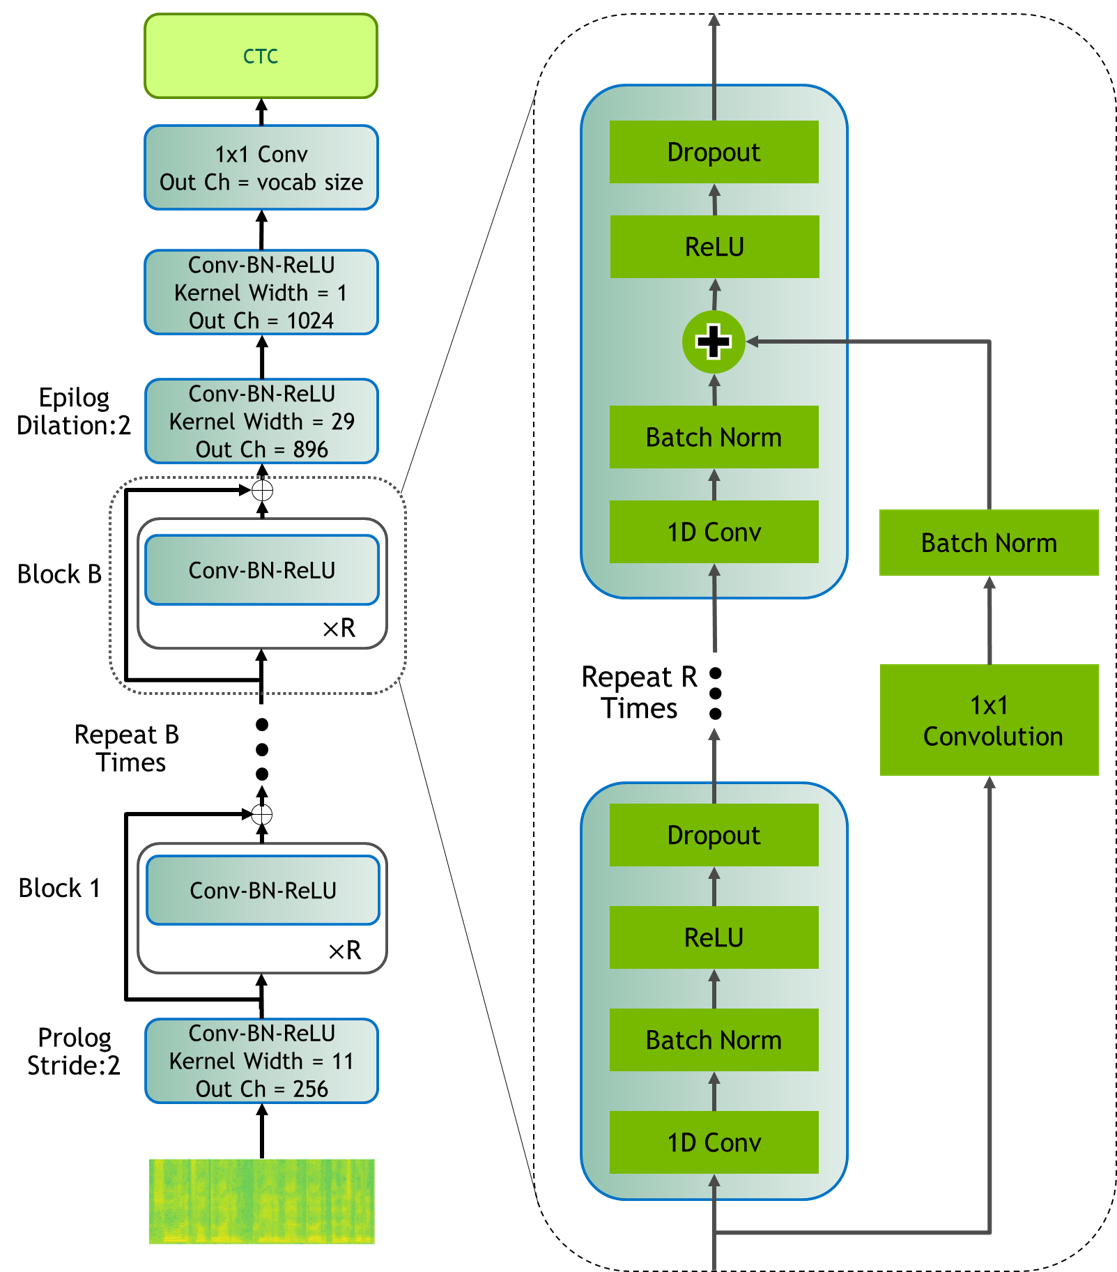
\includegraphics[width=.9\linewidth]{org-download-images/Contribution/2024-08-28_07-44-17_screenshot.png}
\caption{Jasper \(B\times R\) model: \(B\): number of blocks; \(R\): number of sub-blocks.}
\end{figure}
\end{column}
\begin{column}{0.45\columnwidth}
\begin{figure}[htbp]
\centering
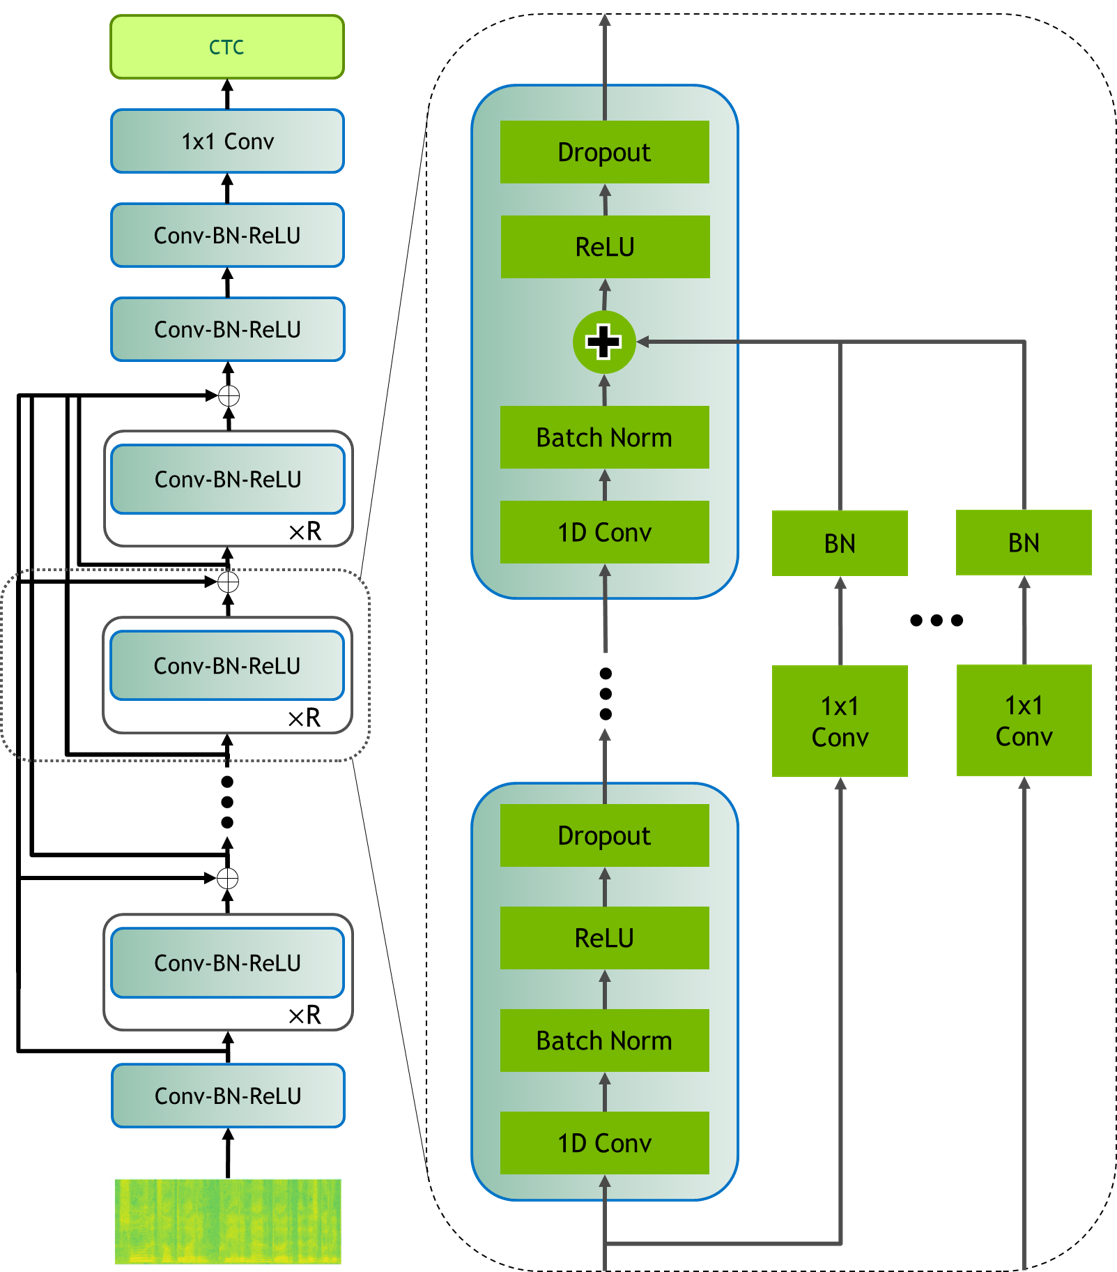
\includegraphics[width=.9\linewidth]{org-download-images/Contribution/2024-08-28_07-46-36_screenshot.png}
\caption{Jasper Dense Residual Model}
\end{figure}
\end{column}
\end{columns}
\end{frame}
\section{quartznet}
\label{sec:org4ac26e5}
\begin{frame}[label={sec:org90d4208}]{quartznet}
solves the same problem as jasper
\end{frame}

\begin{frame}[label={sec:quartznet-architecture}]{quartznet architecture}
\begin{columns}
\begin{column}{.4\columnwidth}
\begin{figure}[htbp]
\centering
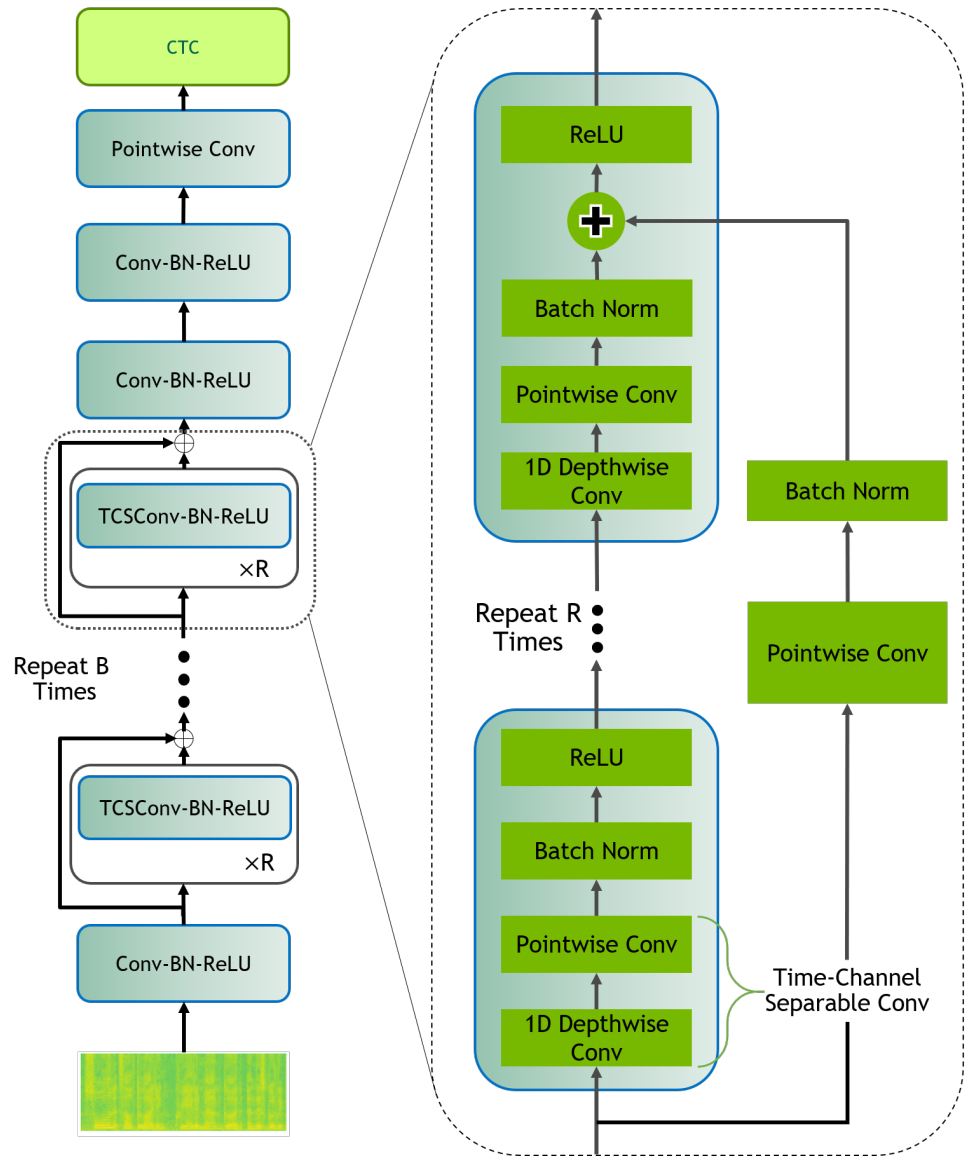
\includegraphics[width=.9\linewidth]{org-download-images/quartznet/2024-10-18_01-36-10_screenshot.png}
\caption{Quartznet Architecture}
\end{figure}
\end{column}
\begin{column}{.6\columnwidth}
\begin{itemize}
\item Uses \alert{separable} conv instead of conv.
\item 1D Conv (along time) \(\to\) 1D Conv (along frequency)
\(\to\) Batch Norm \(\to\) ReLU \\[0pt]
instead of
\item 1D Conv \(\to\) Batch Norm \(\to\) ReLU \(\to\) Dropout.
\end{itemize}
\end{column}
\end{columns}
\end{frame}
\begin{frame}[label={sec:separable-conv}]{separable filters}
\begin{columns}
\begin{column}{.5\columnwidth}
\begin{center}
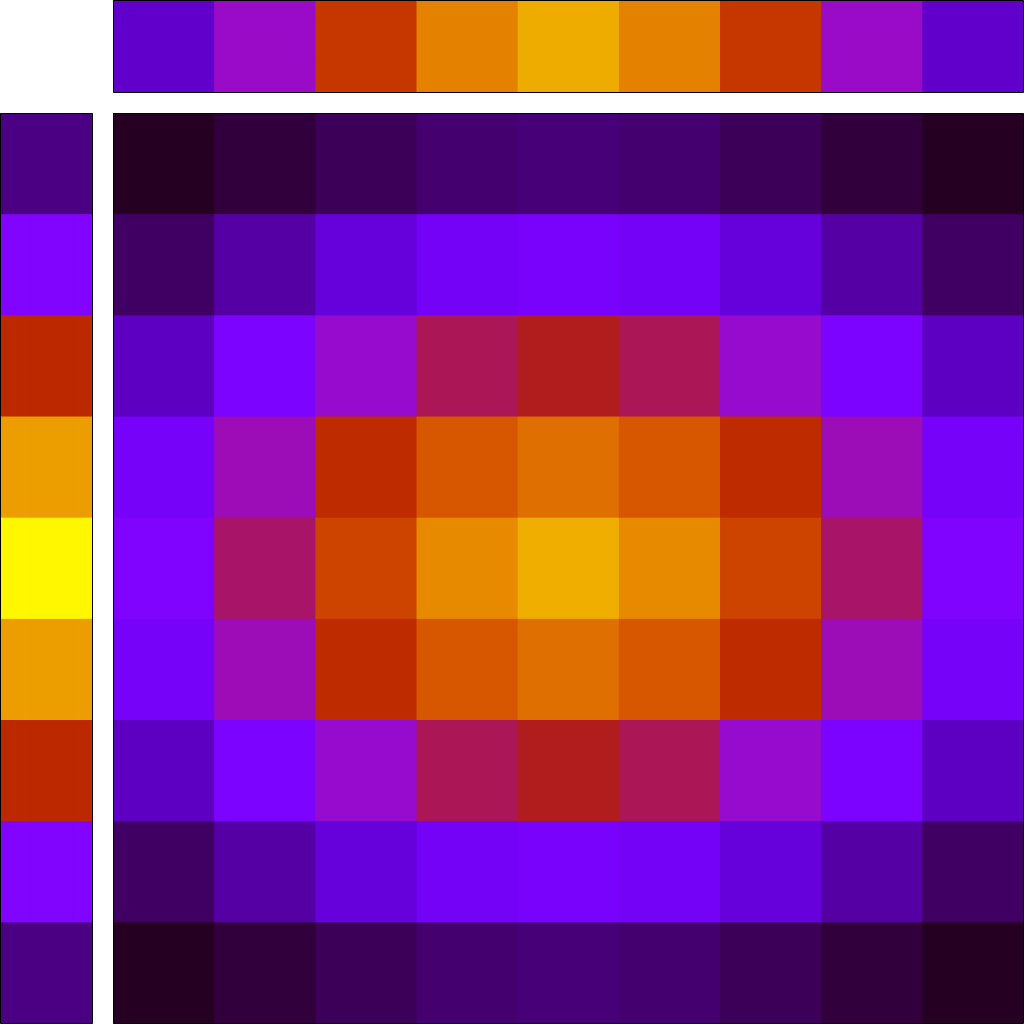
\includegraphics[width=.9\linewidth]{/home/bvraghav/code/tiet-ucs749/tiet-ucs749.github.io/slides/image/sep-conv.png}
\end{center}
\end{column}

\begin{column}{.5\columnwidth}
\(9\times 9\) separable Gaussian filter with constituents
as
\begin{itemize}
\item \(\mathcal{N}(x;0,0.3)\) along the x-axis; and
\item \(\mathcal{N}(y;0,0.15)\) along the y-axis;
\end{itemize}

each resolved within limits \([-1,1]\) into 9 discrete
units.
\end{column}
\end{columns}
\end{frame}

\begin{frame}[label={sec:orgb691388}]{separable filters}
\begin{columns}
\begin{column}{.5\columnwidth}
\begin{center}
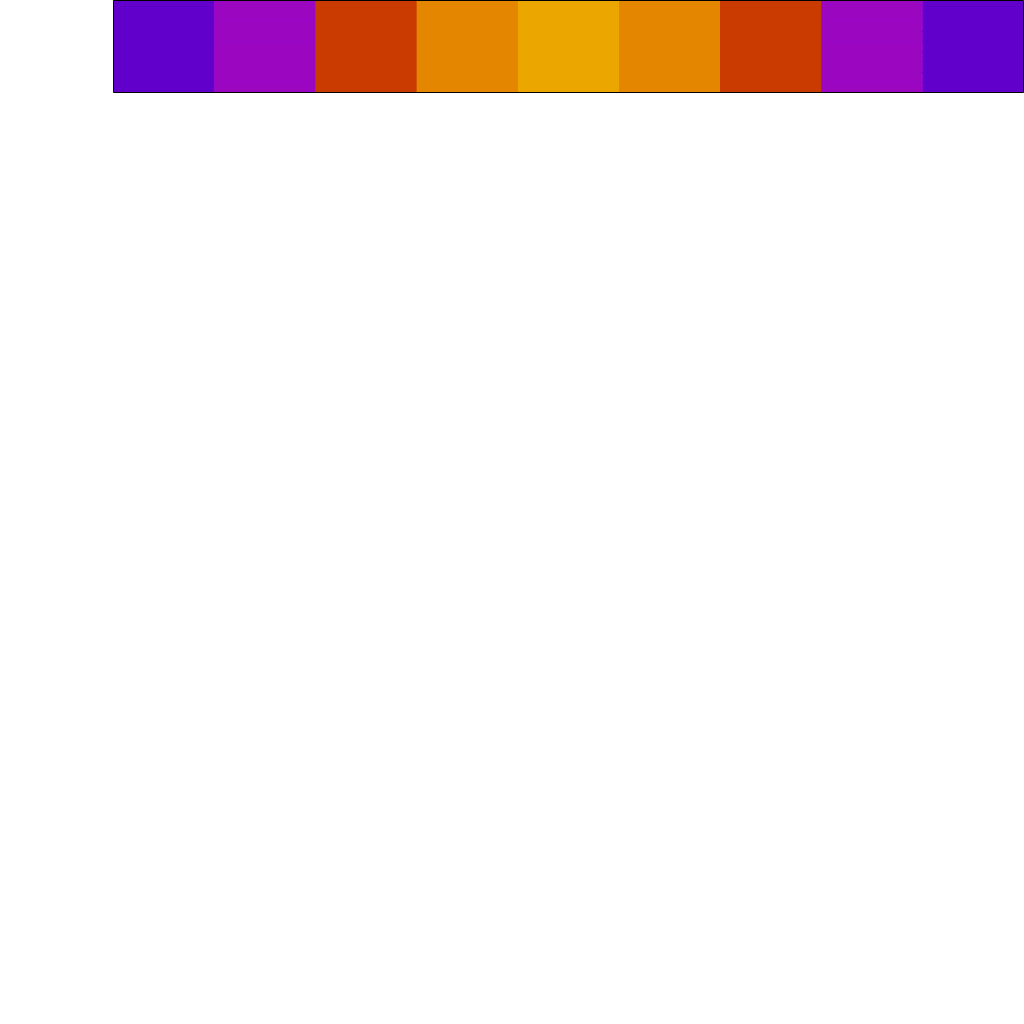
\includegraphics[width=.9\linewidth]{/home/bvraghav/code/tiet-ucs749/tiet-ucs749.github.io/slides/image/sep-conv-fx.png}
\end{center}
\end{column}

\begin{column}{.5\columnwidth}
\begin{align*}
  F_{x} &= \frac{1}{\sqrt{2\pi\sigma^2_x}}
          e^{-\frac{(x-\mu_x)^2}{2\sigma^2_x}}
  \\
  \mu_x &= 5 \qquad \sigma_x = \frac43
\end{align*}
\end{column}
\end{columns}
\end{frame}

\begin{frame}[label={sec:orga275d33}]{separable filters}
\begin{columns}
\begin{column}{.5\columnwidth}
\begin{center}
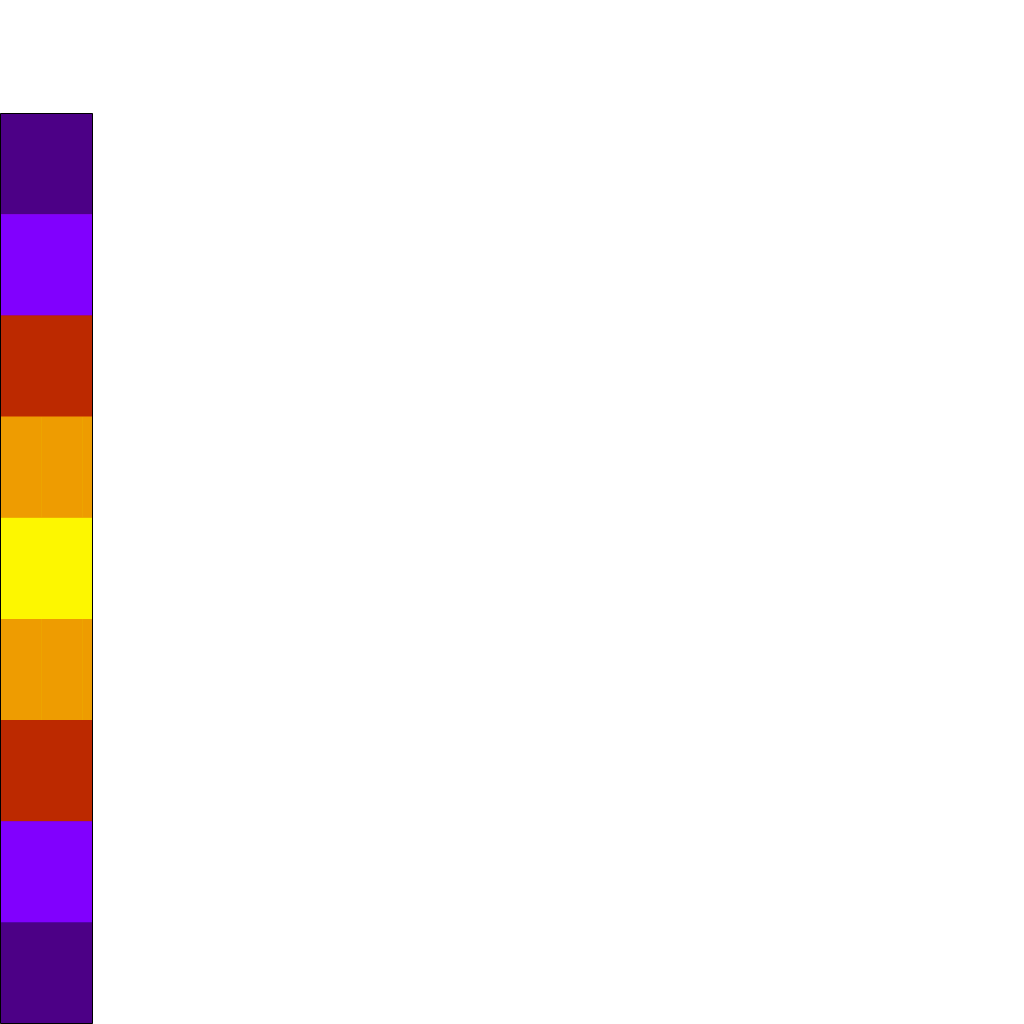
\includegraphics[width=.9\linewidth]{/home/bvraghav/code/tiet-ucs749/tiet-ucs749.github.io/slides/image/sep-conv-fy.png}
\end{center}
\end{column}

\begin{column}{.5\columnwidth}
\begin{align*}
  G_{y} &= \frac{1}{\sqrt{2\pi\sigma^2_y}}
          e^{-\frac{(y-\mu_y)^2}{2\sigma^2_y}}
  \\
  \mu_y &= 5 \qquad \sigma_y = \frac23
\end{align*}
\end{column}
\end{columns}
\end{frame}



\begin{frame}[label={sec:org5a560f6}]{separable filters}
\begin{columns}
\begin{column}{.5\columnwidth}
\begin{center}
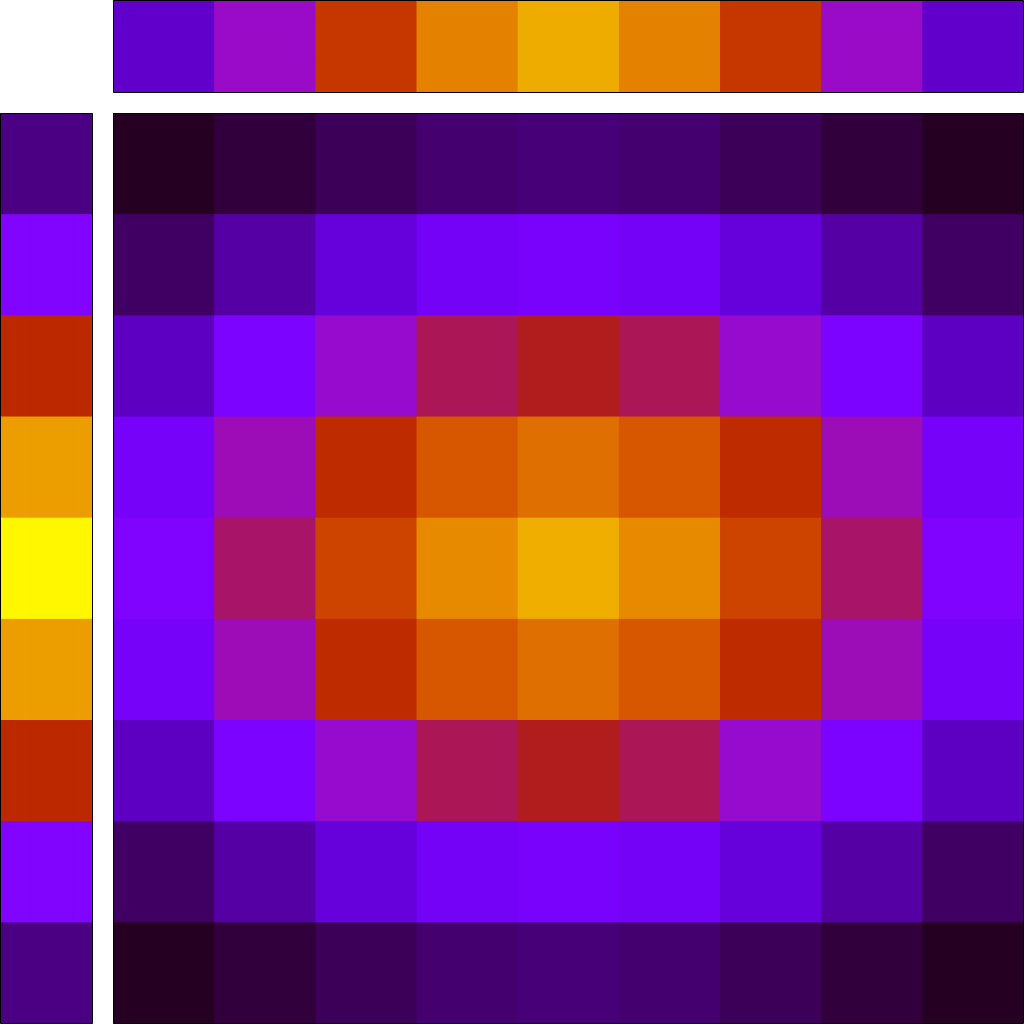
\includegraphics[width=.9\linewidth]{/home/bvraghav/code/tiet-ucs749/tiet-ucs749.github.io/slides/image/sep-conv.png}
\end{center}
\end{column}

\begin{column}{.5\columnwidth}
\begin{align*}
  M_{xy} &= F_x \times G_y
\end{align*}
\end{column}
\end{columns}
\end{frame}


\begin{frame}[label={sec:org5682a5d}]{separable conv}
\begin{columns}
\begin{column}{.5\columnwidth}
\begin{center}
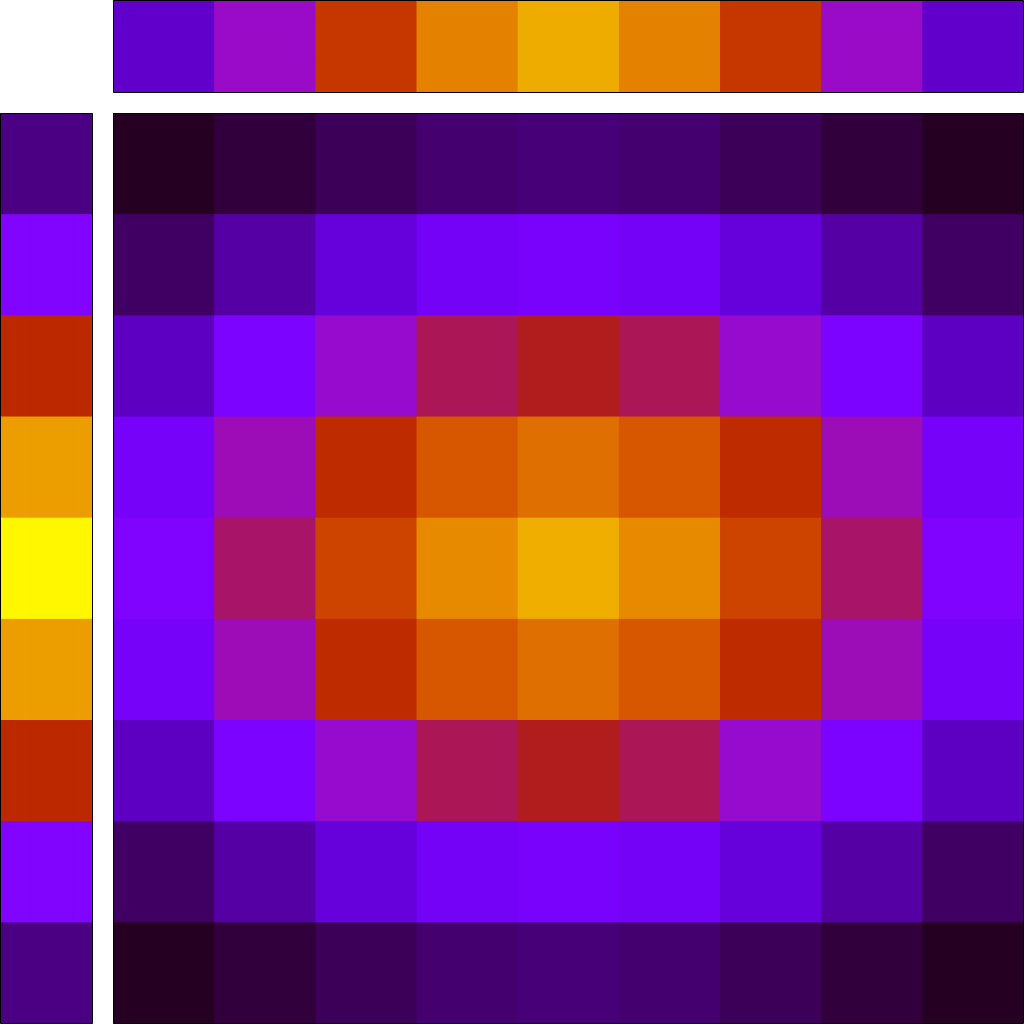
\includegraphics[width=.9\linewidth]{/home/bvraghav/code/tiet-ucs749/tiet-ucs749.github.io/slides/image/sep-conv.png}
\end{center}
\end{column}

\begin{column}{.5\columnwidth}
If \(F\) and \(G\) constitute a separable filter M so that
\(M(x,y)=F(x)\times G(y)\), the following equivalence for
convolution \(\otimes\) over a given signal \(X\), holds
true,

\begin{align*}
  M \otimes X
  &\equiv F \otimes G \otimes X
  \\
  &\equiv G \otimes F \otimes X
\end{align*}
\end{column}
\end{columns}
\end{frame}


\begin{frame}[label={sec:orgaac7e23}]{learnable separable conv}
\begin{columns}
\begin{column}{.5\columnwidth}
\begin{center}
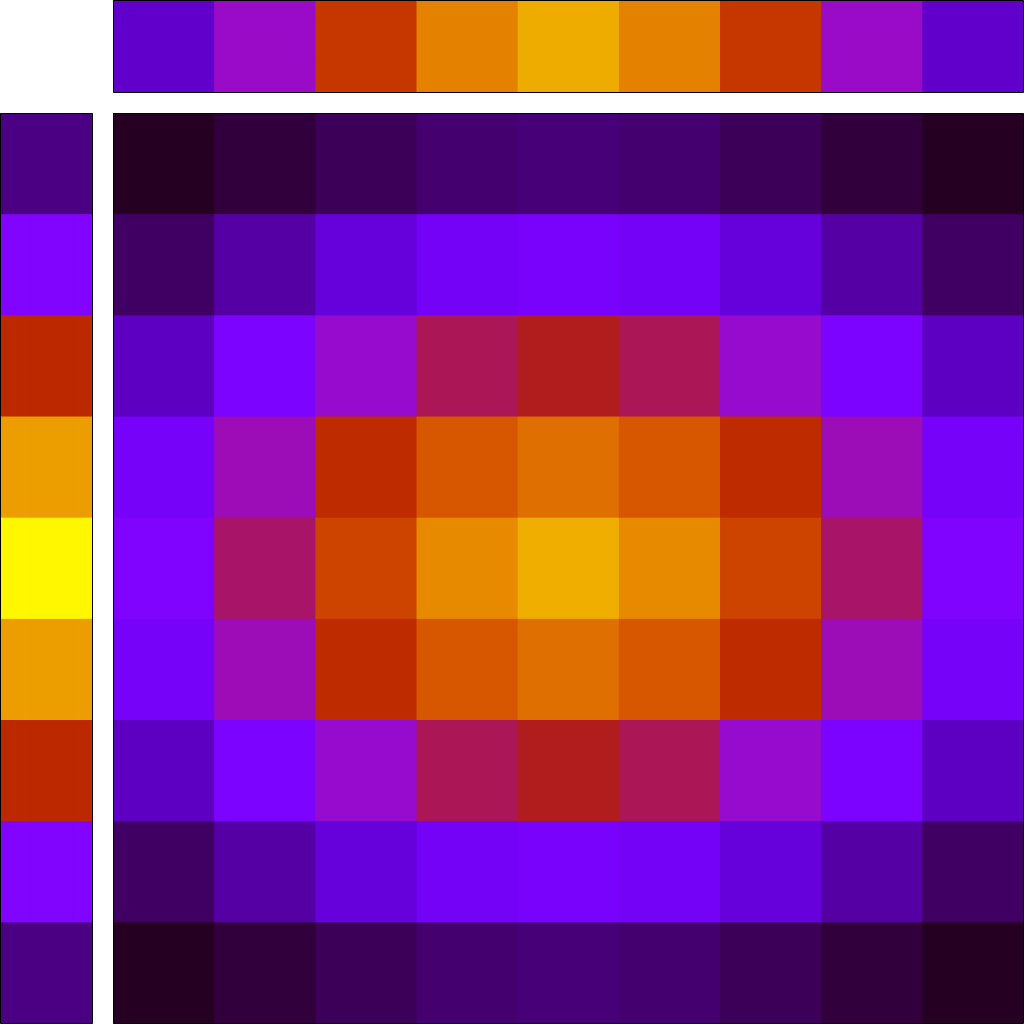
\includegraphics[width=.9\linewidth]{/home/bvraghav/code/tiet-ucs749/tiet-ucs749.github.io/slides/image/sep-conv.png}
\end{center}
\end{column}

\begin{column}{.5\columnwidth}
If \(M\) is a learnable 2D filter with size \(k\times k\);
the num params is \(k^{2}\)

{\vspace{0.3\baselineskip}}

If \(M\) is also separable into \(F\) and \(G\), then, for a
given signal \(X\),

\(M\otimes X \equiv F\otimes G\otimes X\),

with \(F\) and \(G\) bearing \(k\) params each.  Hence, num
params becomes \(2k\).
\end{column}
\end{columns}
\end{frame}

\begin{frame}[label={sec:orgf1d79c9}]{separability in quartznet}
\begin{columns}
\begin{column}{.5\columnwidth}
In Jasper, for a given convolution layer,

\begin{itemize}
\item Let inputs be
\(\mathbf{x}\in\mathbb{R}^{C_{\text{in}}\times t}\);
\item Let outputs be
\(\mathbf{y}\in\mathbb{R}^{C_{\text{out}}\times
  t^{\prime}}\);
\item Let 1D conv filter be of size \(k\);
\item num input time steps \(=t\);
\item num input channels \(=C_{\text{in}}\);
\item num output channels \(=C_{\text{out}}\);
\item num params required for each channel of ouptut
\(=k\times C_{\text{in}}\)
\item num params required in total \(=k\times
  C_{\text{in}}\times C_{\text{out}}\)
\end{itemize}
\end{column}
\begin{column}{.5\columnwidth}
In Quartznet, the same op is implemented in 2 layers,
\begin{itemize}
\item \(F(\mathbf{x})\to\mathbf{y}^{\prime} :
  \mathbf{y}^{\prime}\in\mathbb{R}^{C_{\text{in}}\times
  t^{\prime}}\)
\item \(G(\mathbf{y}^{\prime}) \to \mathbf{y}\)
\item \(F\) convolves over the time axis, separately for each
frequency (input channel); hence num params
\(=k\times C_{\text{in}}\)
\item \(G\) convolves over the frequency axis, with same
kernel for each time step; hence num params
\(=C_{\text{in}}\times C_{\text{out}}\)
\item Total num params \(=k\times C_{\text{in}} +
  C_{\text{in}}\times C_{\text{out}}\)
\end{itemize}
\end{column}
\end{columns}
\end{frame}
\section{citrinet}
\label{sec:org3abab1b}
\begin{frame}[label={sec:orgeb65559}]{citrinet}
solves the same problem as jasper
\end{frame}
\begin{frame}[label={sec:org683768e}]{citrinet architecture}
\begin{columns}
\begin{column}{0.45\columnwidth}
\only<+>{
\begin{center}
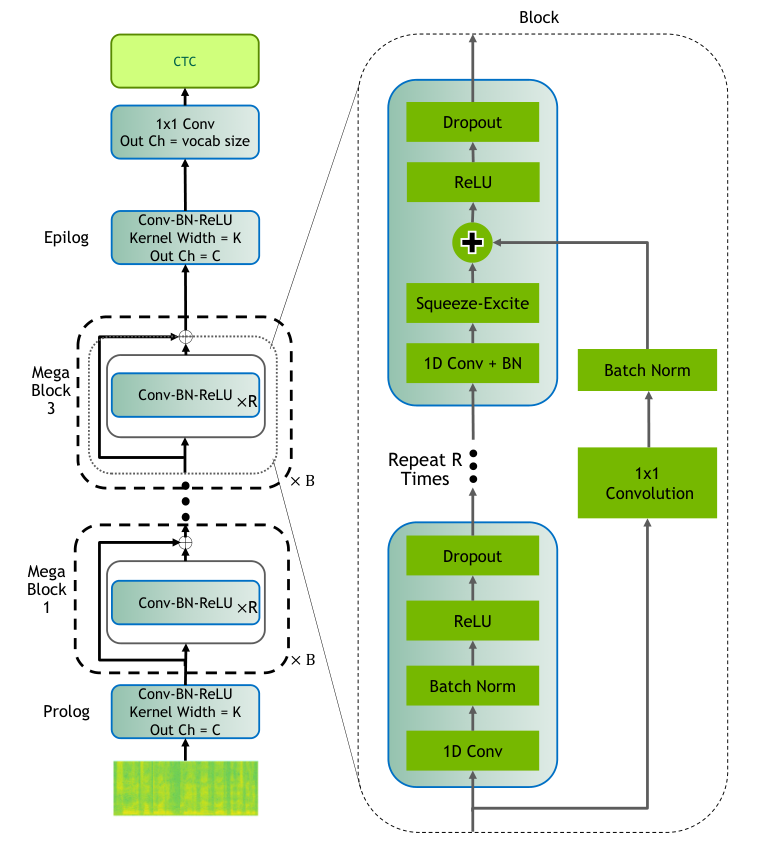
\includegraphics[width=.9\linewidth]{org-download-images/citrinet/2024-11-19_09-32-01_screenshot.png}
\end{center}
}\only<+->{

\begin{center}
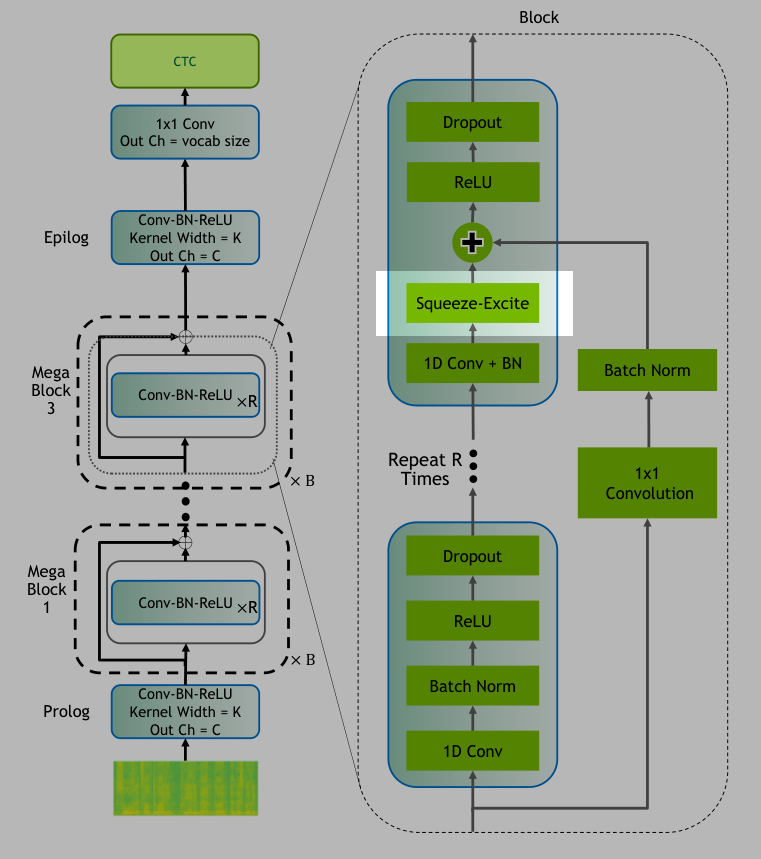
\includegraphics[width=.9\linewidth]{org-download-images/citrinet/2024-11-19_09-37-34_screenshot.png}
\end{center}

}
\end{column}

\begin{column}{.55\columnwidth}
Uses \alert{squeeze and excitation} attention on top of
\emph{conv + bn} and before non-linear activation.

\begin{align*}
  \mathrm{SE}\;(\mathbf{x})
  &= \mathbf{x} \otimes F_{sc}\circ F_{ex}\circ F_{sq}
    (\mathbf{x}) 
\end{align*}

where, \(\otimes\) is the Hadamard product (element-wise
product)

\alert{Conv} is Time–channel separable Conv as in Quartznet.
\end{column}
\end{columns}
\end{frame}

\begin{frame}[label={sec:org99b821d}]{squeeze and excitation}
\begin{align*}
  \mathrm{SE}\;(\mathbf{x})
  &= \mathbf{x} \otimes F_{sc}\circ F_{ex}\circ F_{sq}
    (\mathbf{x}) 
\end{align*}

\begin{center}
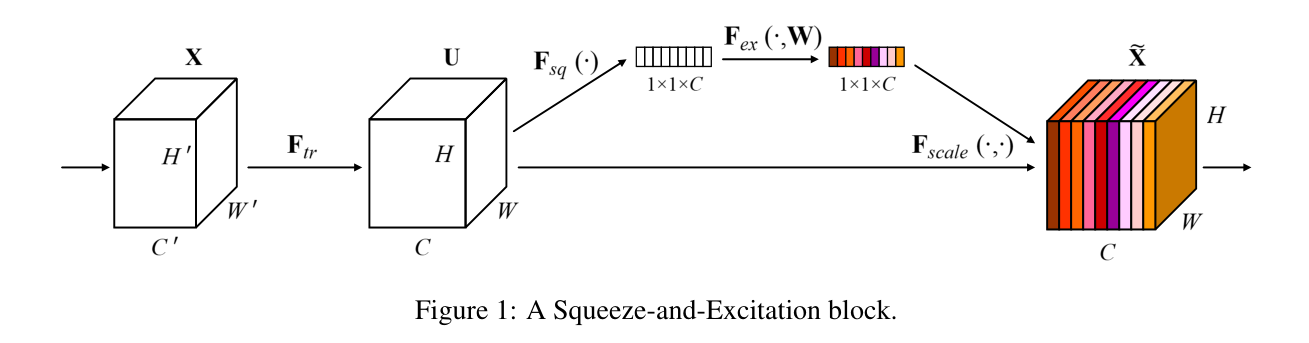
\includegraphics[width=.9\linewidth]{org-download-images/citrinet/2024-11-19_09-55-43_screenshot.png}
\end{center}

\scriptsize The image is from the original
squeeze and excitation paper; and shows \(\mathrm{SE}\)
in the context of 2D Conv.  But recall that in the
context of speech recognition we have 1D Conv; and the
same concept is extended trivially.
\end{frame}

\begin{frame}[label={sec:orga9f98b7}]{squeeze and excitation}
\begin{center}
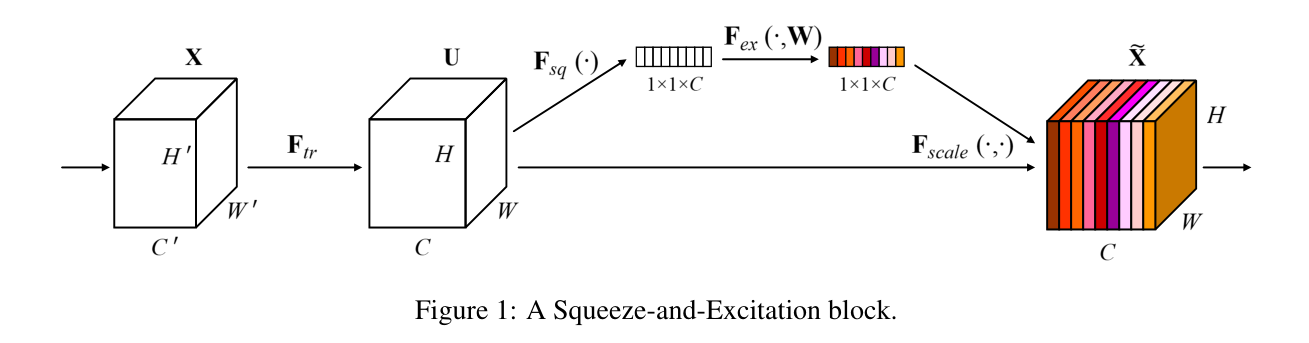
\includegraphics[width=.9\linewidth]{org-download-images/citrinet/2024-11-19_09-55-43_screenshot.png}
\end{center}

\begin{description}
\item[{\(F_{sq} (\mathbf{x}) = \bar{\mathbf{x}} = \frac1T\sum_t\mathbf{x}_t\)}] performs global average pooling; \(\to 1\times C\)
\item[{\(F_{ex} (\mathbf{x}) = \mathrm{RELU}(W_1\mathbf{x} + \mathbf{b}_1)\)}] conv+RELU; \(1\times C\to1\times c\); typically \(c<C\);
\item[{\(F_{sc} (\mathbf{x}) = \mathrm{sigmoid}(W_2\mathbf{x} + \mathbf{b}_2)\)}] conv+sigmoid; \(1\times c \to 1\times C\);
\end{description}
\end{frame}

\begin{frame}[label={sec:orgf9dd878}]{results}
\begin{columns}
\begin{column}{.4\columnwidth}
\begin{center}
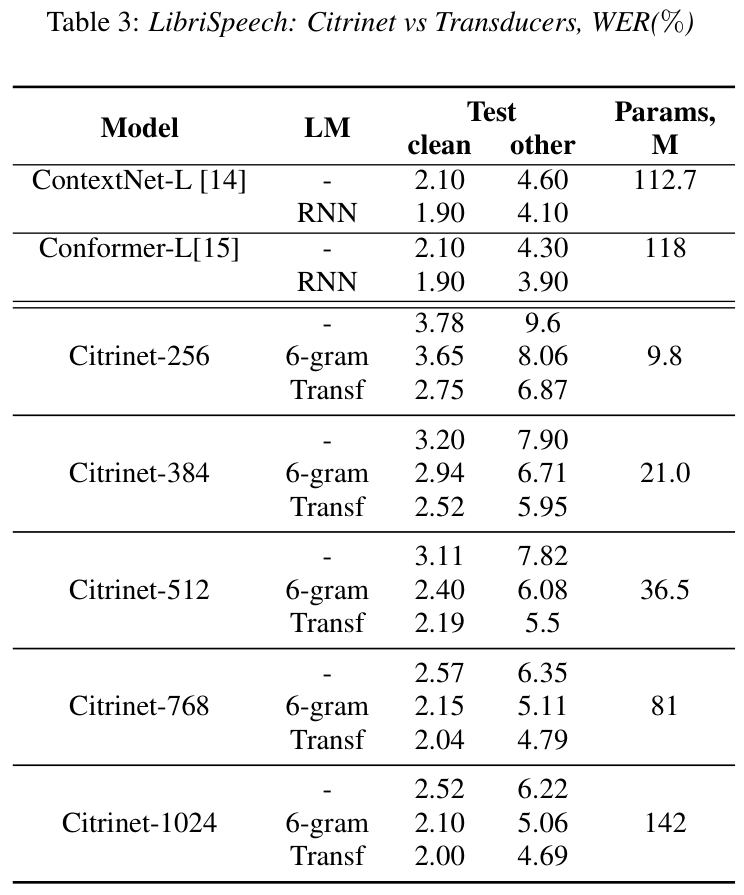
\includegraphics[width=.9\linewidth]{org-download-images/citrinet/2024-11-19_10-44-03_screenshot.png}
\end{center}
\end{column}

\begin{column}{.6\columnwidth}
Citrinet shows comparable performance with
significantly lower number of params.
\end{column}
\end{columns}
\end{frame}

\section{matchboxnet}
\label{sec:orgd2a5694}

\begin{frame}[label={sec:org39d11e0}]{matchboxnet}
\begin{itemize}
\item Uses a similar architecture as jasper for keyword
spotting aka speech command recognition;

\item Designed for devices with low computational and
memory resources;

\item SoTA performance with significantly fewer params.
\end{itemize}

Also,

\begin{itemize}
\item Fixed length input (1 second long utterance).
\end{itemize}
\end{frame}

\begin{frame}[label={sec:orgeb3f51f}]{matchboxnet architecture}
\begin{columns}
\begin{column}{0.45\columnwidth}
\only<+>{

\begin{center}
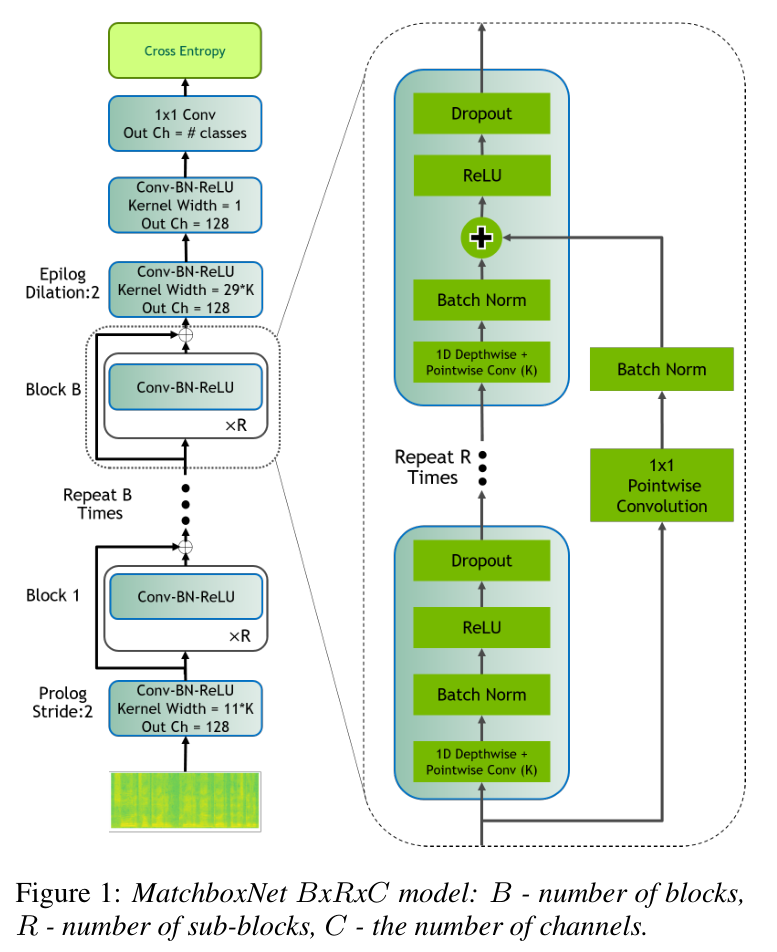
\includegraphics[width=.9\linewidth]{org-download-images/matchboxnet/2024-11-19_11-11-19_screenshot.png}
\end{center}

} \only<+>{

\begin{center}
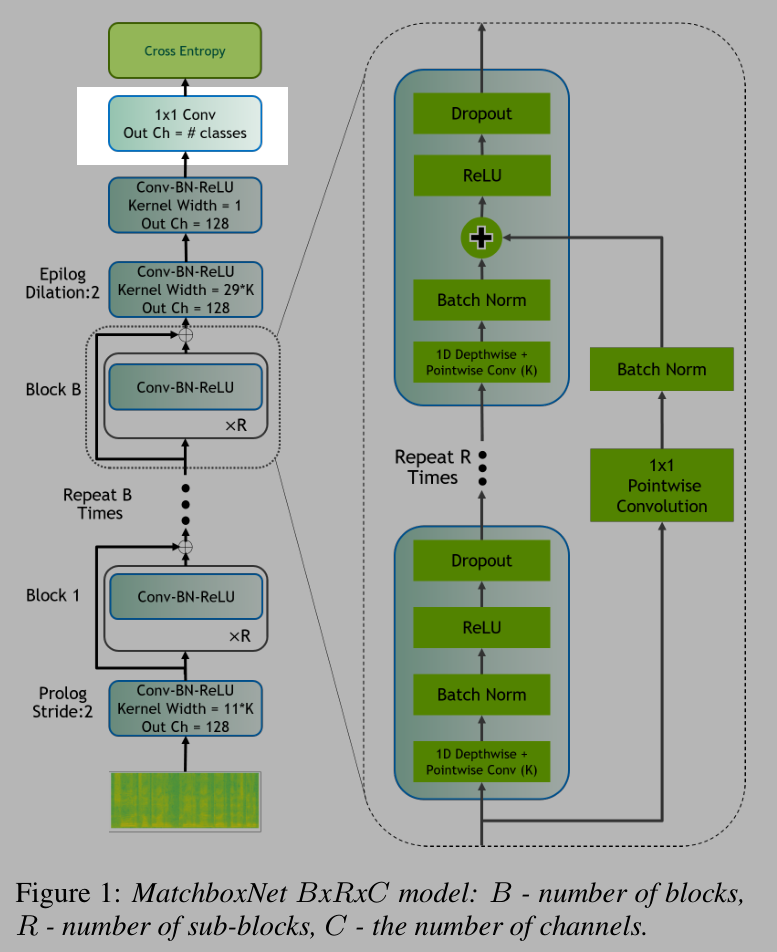
\includegraphics[width=.9\linewidth]{org-download-images/matchboxnet/2024-11-19_11-12-42_screenshot.png}
\end{center}
}
\end{column}

\begin{column}{.55\columnwidth}
\begin{center}
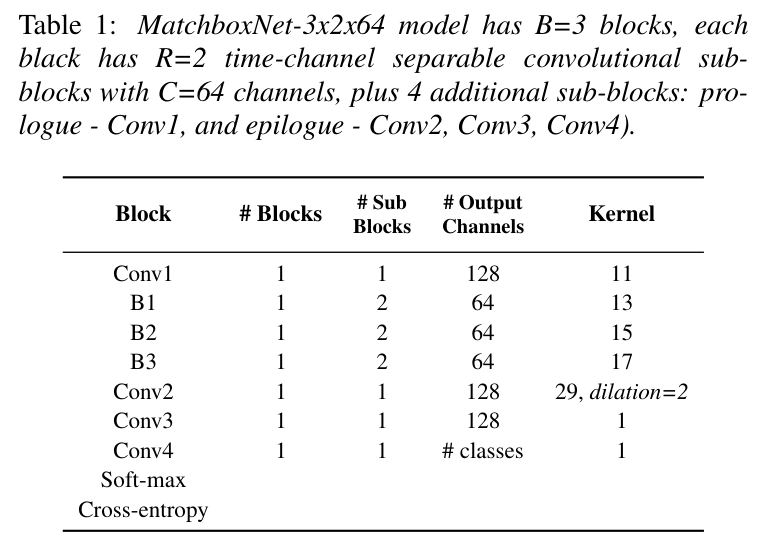
\includegraphics[width=.9\linewidth]{org-download-images/matchboxnet/2024-11-19_11-14-11_screenshot.png}
\end{center}
\end{column}
\end{columns}
\end{frame}

\begin{frame}[label={sec:org43e6829}]{results}
\begin{columns}
\begin{column}{0.45\columnwidth}
\begin{center}
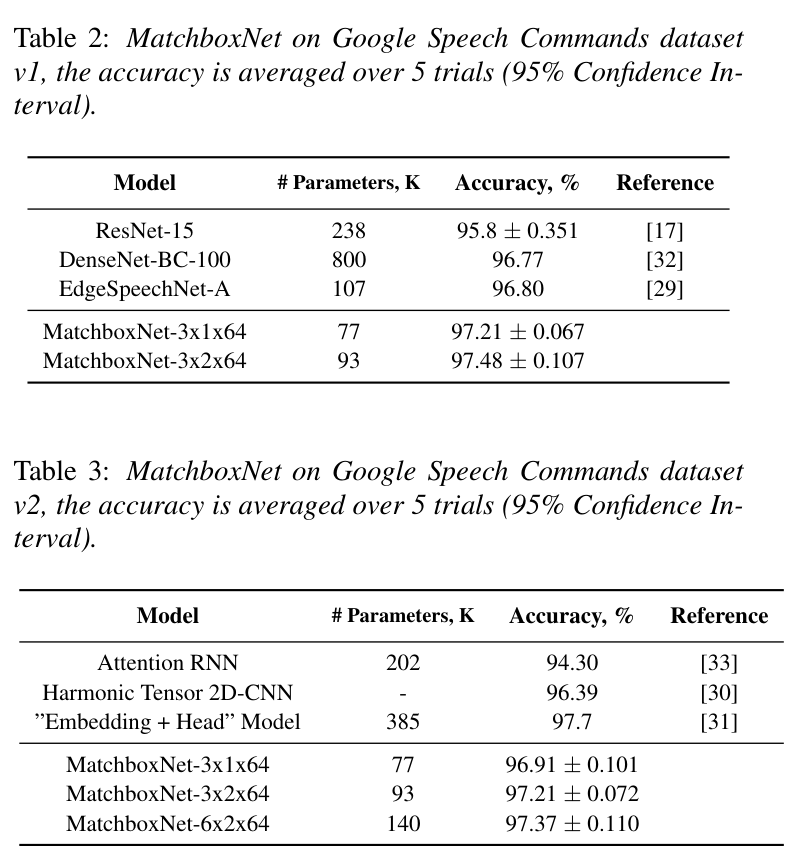
\includegraphics[width=.9\linewidth]{org-download-images/matchboxnet/2024-11-19_11-19-19_screenshot.png}
\end{center}
\end{column}
\end{columns}
\end{frame}
\end{document}
